\documentclass[titlepage, a4paper]{article}
\usepackage[english]{babel}
\usepackage[utf8]{inputenc}
\usepackage{graphicx}
\usepackage{color}
\usepackage{mathtools}
\usepackage{float}
\usepackage[parfill]{parskip}
\usepackage[margin=10pt,font=small,labelfont=bf,labelsep=endash]{caption}
\usepackage{epstopdf}
\usepackage{listings}
\usepackage{enumitem}
\usepackage{soul}
\epstopdfsetup{suffix=}
\DeclareGraphicsExtensions{.ps}
\DeclareGraphicsRule{.ps}{pdf}{.pdf}{`ps2pdf -dEPSCrop -dNOSAFER #1 \noexpand\OutputFile}

\lstset{literate=%
    {å}{{\r{a}}}1
    {ä}{{\"a}}1
    {ö}{{\"o}}1
    {Å}{{\r{A}}}1
    {Ä}{{\"A}}1
    {Ö}{{\"O}}1
}

\newcommand{\todo}[1] {\textbf{\textcolor{red}{#1}}}

\usepackage{fancyhdr}
\fancyhead[L]{}
\pagestyle{fancy}
\rhead{Pål Kastman \\ Alexander Yngve}
\chead{TDTS08}
\thispagestyle{empty}

\begin{document}

{\ }\vspace{45mm}

\begin{center}
  \Huge \textbf{TDTS08: whattolearn}
\end{center}

\vspace{250pt}

\begin{center}
  \begin{tabular}{|*{3}{p{40mm}|}}
    \hline
    \textbf{Name} & \textbf{PIN} & \textbf{Email} \\ \hline
           {Pål Kastman} & {851212-7575} & {palka285@student.liu.se} \\ \hline
           {Alexander Yngve} & {930320-6651} & {aleyn573@student.liu.se} \\ \hline
  \end{tabular}
\end{center}
\newpage

\tableofcontents
\thispagestyle{empty}
\newpage

\section{Introduction}
This documents only purpose is to document what I will need to learn in the course tdts08. \\
\todo{YNGVE OM DU VILL BYTA RUBRIKERNA SÅ ÄR DET HELT OKEJ, DOM ÄR BARA DÄR SOM STÖD NU}

\section{Lecture 2: Memory Systems}

\textbf{Sequential access}: Memory is organized into units of data, called records. Access must be made in a specific linear sequence. Stored addressing information is used to separate records and assist in the retrieval process. A shared read–write mechanism is used, and this must be moved from its current location to the desired location, passing an rejecting each intermediate record. Thus, the time to access an arbitrary record is highly variable. \textbf{Tape units}  are sequential access.

\textbf{Direct access}: As with sequential access, direct access involves a shared read–write mechanism. However, individual blocks or records have a unique address based on physical location. Access is accomplished by direct access to reach a general vicinity plus sequential searching, counting, or waiting to reach the final location. Again, access time is variable. \textbf{Disk units} are direct access.

\textbf{Random access}: Eacha ddressable location inm emory has a unique, physically wired-in addressing mechanism. The time to access a given location is inde- pendent of the sequence of prior accesses and is constant. Thus, any location can be selected at random and directly addressed and accessed. Main memory and some cache systems are random access.

\textbf{Associative}: This is arandom access type of memory that enables one to make a comparison of desired bit locations within a word for a specified match, and to do this for all words simultaneously. Thus, a word is retrieved based on a portion of its contents rather than its address.

\textbf{Access time (latency)}: For random-access memory, this is the time it takes to perform a read or write operation, that is, the time from the instant that an address is presented to the memory to the instant that data have been stored or made available for use. For non-random-access memory, access time is the time it takes to position the read–write mechanism at the desired location.

\textbf{Transfer rate}: This is the rate at which data can be transferred into or out of a memory unit. For random-access memory, it is equal to 1/(cycle time).
For non-random-access memory, the following relationship holds:

$$T_n = T_A + \frac{n}{R}$$

$T_n$ = Average time to read or write n bits \\
$T_A$ = Average access time \\
$n$ = Number of bits \\
$R$ = Transfer rate, in bits per second (bps) \\

\subsection{Memory hierarchy}
\textbf{Registers} Built into the processors, very small and expensive. \\
\textbf{Main Memory} Memory that the cache collects data from. \\
\textbf{Secondary Memory (of direct access type)} Bigger in size, but less expensive per Byte. \\
\textbf{Secondary Memory (of archive type)} And so on. \\



\subsection{Cache memory}
There is a big gap in speed between register and main memory, this is why we need to use cache memory.

Cache memory is designed to combine the memory access time of expensive, high-speed memory combined with the large memory size of less expensive, lower-speed memory.
ller, faster cache memory.

The cache contains a copy of portions of main memory. When the processor attempts to read a word of memory, a check is made to determine if the word is in the cache. If so, the word is delivered to the processor. If not, a block of main memory, consisting of some fixed number of words, is read into the cache and then the word is delivered to the processor.

We would like the size of the cache to be small enough so that the overall average cost per bit is close to that of main memory alone and large enough so that the overall average access time is close to that of the cache alone.




\subsubsection{Locality of reference}
The intermediate-future memory access will usually refer to the same word or words in the neighborhood, and will not have to involve the main memory.

\textbf{Temporal Locality} -- If an item is referenced, it will tend to be referenced again in the near future. \\
\textbf{Spatial Locality} -- If an item is referenced, items whose addresses are close by will tend to be referenced soon. \\

\subsubsection{Replacement methods}
yes, there's different kinds of them.

\subsubsection{Cache Design}

One, two, three level caches, how does it work. up- and downsides of them.

\textbf{Split Caches} means that we have separate caches for instructions and data. \\
+ Competition for the cache between instruction and data is eliminated \\
+ Instruction fetch can proceed in parallel with memory access from the CPU for operands. \\
- One may be overloaded while the other is under utilized. \\

\textbf{Unified Caches} means that both instructions and data uses the same cache.
+ Better balance the load between instruction and data fetches depending on the dynamics of the program execution. \\
+ Design and implementation are cheaper. \\
-- Lower performance. \\
\subsubsection{Direct mapping cache}
Each block of the main memory is mapped into a fixed cache slot. \\
+ Simple to implement and therefore inexpensive. \\
-- If a program accesses 2 blocks that map to the same cache slot repeatedly, cache miss rate is very high. \\

\subsubsection{Associative mapping cache}
A main memory block can be loaded into any slot of the cache. To determine if a block is in the cache, a mechanism is needed to simultaneously examine every slot’s tag. In this case, the cache control logic interprets a memory address simply as a Tag and a Word field. The Tag field uniquely identifies a block of main memory. To determine whether a block is in the cache, the cache control logic must simultaneously examine every line’s tag for a match. \\

The downside of this is the complex circuitry needed to examine all the tags.

\subsubsection{Set Associative mapping cache}
A fully associative mapped memory can be built but is very expensive, and therefore is not done. Instead we use a \textbf{set associative} cache memory. \\
Here the cache are divided into a number of sets, where each set contains a number of slots (just like a regular cache). 


\subsubsection{Fully Associative Organization}


\subsubsection{Write Policy}
When a block in the cache is to be replaced, we have to consider two cases. If the block in the case has \textbf{not been altered}, then it can be replaced with a new block without saving the block to the main memory. Or if it \textbf{has been altered} (one block is enough), then we need to write that block back to main memory. \\

There are two cases to consider
\begin{enumerate}
\item More than one device may have access to main memory. \\
  
  For example, an I/O module may be able to read-write directly to memory. If a word has been altered only in the cache, then the corresponding memory word is invalid. Further, if the I/O device has altered main memory, then the cache word is invalid. \\
\item Multiple processors are attached to the same bus and each processor has its own local cache. Then, if a word is altered in one cache, it could conceivably invalidate a word in other caches.
\end{enumerate}
\textbf{Write through} all write operations are made to main memory as well as to the cache, ensuring that main memory is always valid. Any other processor–cache module can monitor traffic to main memory to maintain consistency within its own cache. The main disadvantage of this technique is that it generates substantial memory traffic and may create a bottleneck.\\

\textbf{Write through with buffered write} The same as write-through, but instead of slowing the processor down by writing directly to main memory, the write address and data
are stored in a high-speed write buffer; the write buffer transfers data to main memory while the processor continues its task.\\

\textbf{Write back} With write back, updates are made only in the cache. When an update occurs, a dirty bit, or use bit, associated with the line is set. Then, when a block is replaced, it is written back to main memory if and only if the dirty bit is set. \\

\subsection{Virtual memory}
Almost all nonembedded processors, and many embedded processors, support virtual memory. In essence, virtual memory is a facility that allows programs to address memory from a logical point of view, without regard to the amount of main memory physically available. When virtual memory is used, the address fields of machine instructions contain virtual addresses. For reads to and writes from main memory, a hardware memory management unit (MMU) translates each virtual address into a physical address in main memory.

\subsubsection{Paging}
Unequal fixed-size and variable-sized partitions of memory are inefficient, we need to make sure that we use the most of the memory available in the best way, we try to do this using pages.

We first divide programs into fixed sized memory blocks called pages, then we divide the main memory into equal fixed sized blocks, called page frames. \\

A process then needs a set of free page frames assigned by the OS. Then its up to the OS to make sure it keeps track of the free available frames, it also uses a page table to keep track of the mapping between pages and page frames. 

\subsubsection{Page fault}
When we try to access a piece of memory that is not currently in the main memory, but instead in the virtual memory. The OS must then load the page into the main memory firs, this is called a \textbf{Page fault}.

\subsubsection{Page replacement}
When a page fault occurs and all the page frames are occupied, one of them must be replaced. If the page that are to be replaced, has been modified, we need to write that memory back to the secondary storage. \\

We want to replace a page that we think will not be accessed for the longest amount of time. The problem is that we can't predict the future, so we have to predict the future, we can do this in some different ways, described below.

\subsubsection{Replacement algorithms}
Not needed with direct mapping, but with associative mapping we need one of these algorithms. \\

\textbf{First-in-first-out} \\
\textbf{Least recently used (LRU)}: replaces the cache that has been in the cache the longest without being referenced.\\
\textbf{Least frequently used (LFU)}: replaces the cache that has been referenced the least frequent.\\ 
\textbf{Random}\\ 

\newpage
\section{Lecture 3: Instruction pipelining}
The idea is to divide the workload into different stages, so that we don't have to wait for an instruction to complete before we fetch the next one.

The typical pipeline has \textbf{six} stages: \\
1. Fetch Instruction (FI): Fetch the instruction.\\
2. Decode Instruction (DI): Determine the op-code and the operand specifiers.\\
3. Calculate Operands (CO): Calculate the effective addresses.\\
4. Fetch Operands (FO): Fetch the operands.\\
5. Execute Instruction (EI): perform the operation.\\
6. Write Operand (WO): store the result in memory.\\

The ideal case gives us a speed-up of six times. But in practice we have some problems.

In general, a larger number of stages gives better performance. \\
However, a large number also increases the complexity. We have to  move a lot of information between stages, and synchronize the stages. We call the problems that occur \textbf{Pipeline Hazards}.

\subsection{Pipeline hazards}
There are different kinds of pipeline hazards, first we have the case with dependency, A pipeline hazard occurs when the pipeline, or some portion of the pipeline, must stall because conditions do not permit continued execution. Such a pipe- line stall is also referred to as a pipeline bubble. There are three types of hazards: resource, data, and control. \\

\subsubsection{Structural (resource) hazards}
A \textbf{Resource hazards} resource hazard occurs when two (or more) instructions that are already in the pipeline need the same resource. The result is that the instructions must be executed in serial rather than parallel for a portion of the pipeline. A resource hazard is sometime referred to as a structural hazard.

\subsubsection{Data hazards}
A \textbf{Data Hazard} is when two instructions in a program are to be executed in sequence and both access a particular memory or register operand. If the two instructions are executed in strict sequence, no problem occurs. However, if the instructions are executed in a pipeline, then it is possible for the operand value to be updated in such a way as to produce a different result than would occur with strict sequential execution.

There are three types of data hazards: \\
• Read after write (RAW), or true dependency: An instruction modifies a reg- ister or memory location and a succeeding instruction reads the data in that memory or register location. A hazard occurs if the read takes place before the write operation is complete. \\
• Write after read(WAR), or antidependency: Aninstructionreadsaregisteror memory location and a succeeding instruction writes to the location. A hazard occurs if the write operation completes before the read operation takes place. \\
• Write after write (WAW), or output dependency: Two instructions both write to the same location. A hazard occurs if the write operations take place in the reverse order of the intended sequence. \\

We can handle this by using a technique called forwarding (bypassing). This works in the following way: \\
The ALU passes its result back into a MUX. If this detects that the value have been updated and not yet written back into the main memory, the value from the ALU will be used instead of the value we fetched from the memory as can be seen in figure \ref{fig:bypassing}.

\begin{figure}[H]
	\centering
	\scalebox{0.342}{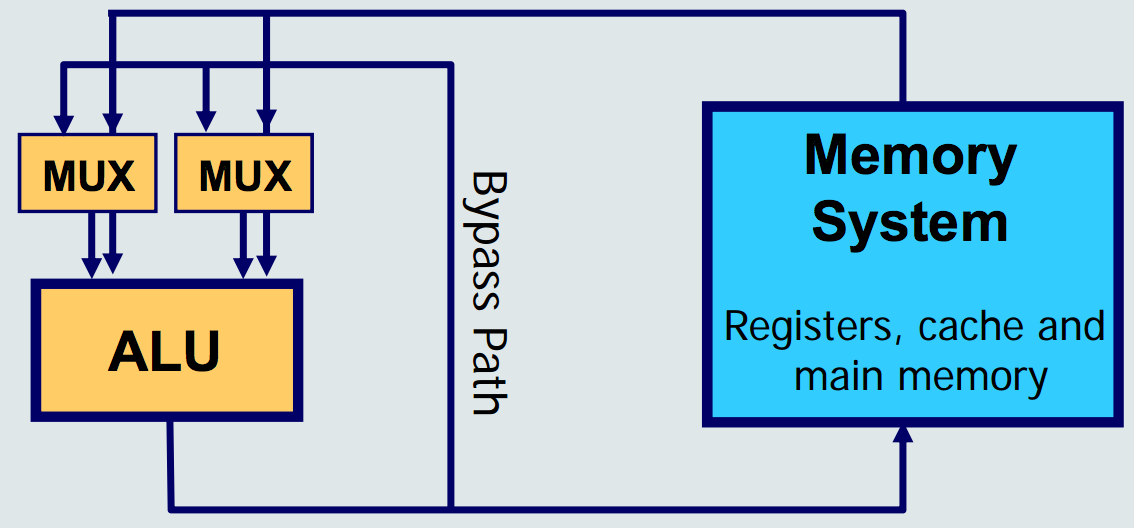
\includegraphics{img/bypassing.png}}
	\caption{The ALU passes its calculated value back into a MUX.}
	\label{fig:bypassing}
\end{figure}

\subsubsection{Control hazards}
A \textbf{control hazard}, also known as a branch hazard, occurs when the pipeline makes the wrong decision on a branch prediction and therefore brings instructions into the pipeline that must subsequently be discarded as seen in figure \ref{fig:control-hazard}.

\begin{figure}[H]
	\centering
	\scalebox{0.342}{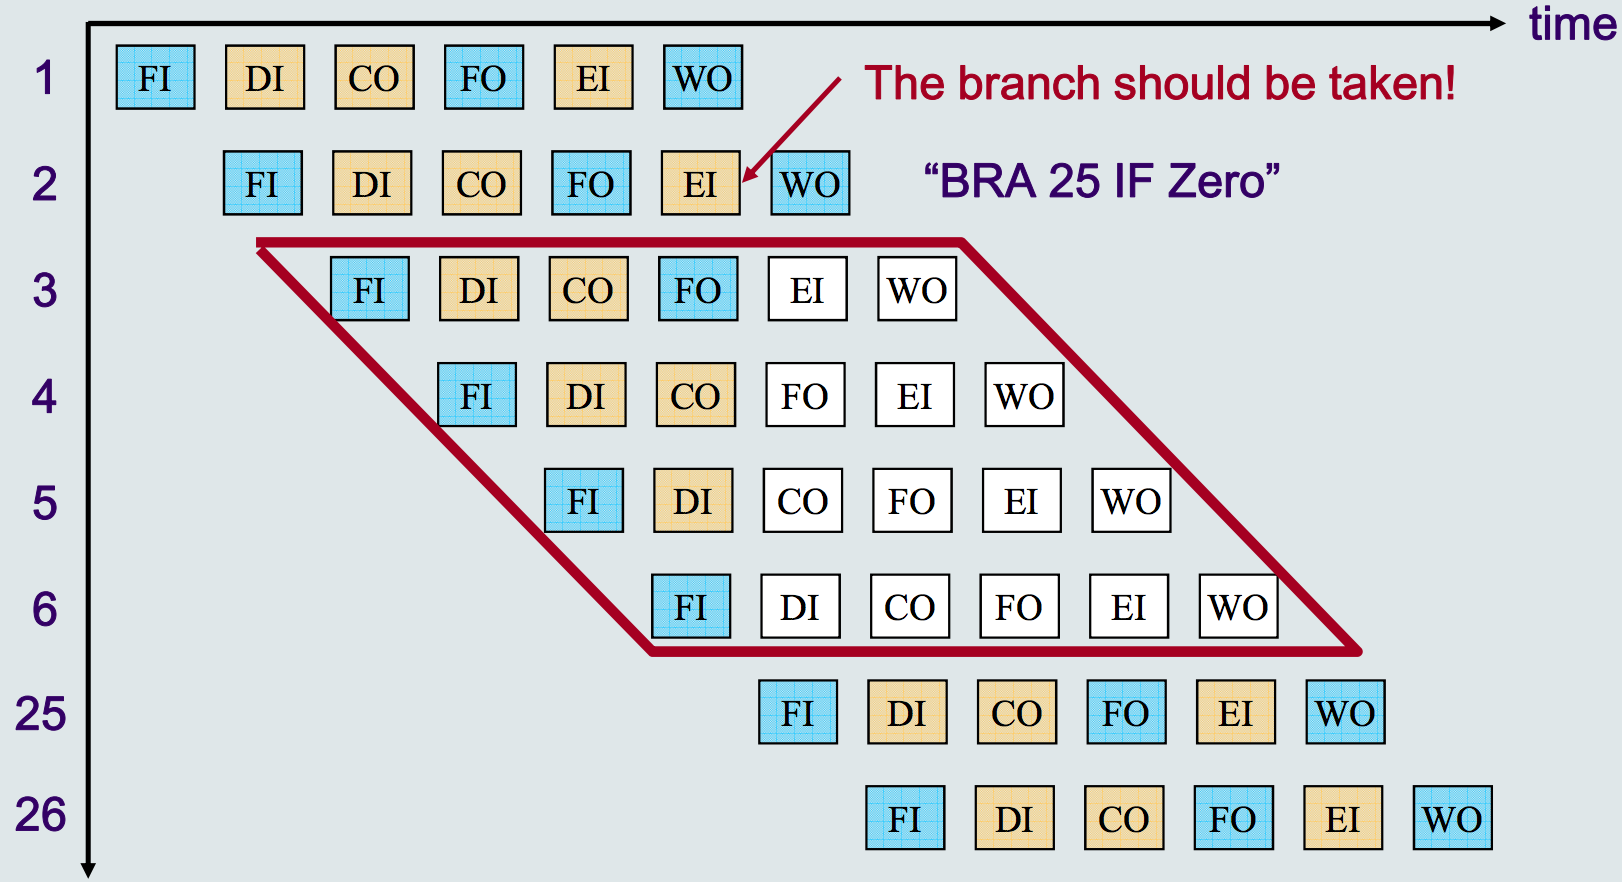
\includegraphics{img/control-hazard.png}}
	\caption{Control hazards.}
	\label{fig:control-hazard}
\end{figure}


\subsection{Branch handling}
There are different ways of handling branches. \\

\subsubsection{Stop the pipeline}
We can stall all the next instructions until the current branch reaches its final stage and we know what to do, this is expensive due to that 20-35\% of the things instructions executed are executed as branches.

\subsubsection{Multiple streams}
Implement hardware resources so that we can execute both alternatives in parallel, there are two problems with this though:
\begin{enumerate}
\item With multiple pipelines there are contention delays for access to the registers and to memory. \\
\item Additional branch instructions may enter the pipeline (either stream) before the original branch decision is resolved. Each such instruction needs an addi- tional stream.
\end{enumerate}

\subsubsection{Pre-fetch branch target}
When a conditional branch is recognized, the target of the branch is prefetched, in addition to the instruction following the branch. This target is then saved until the branch instruction is executed. If the branch is taken, the target has already been prefetched.

\subsubsection{Loop buffer}
A loop buffer is a small, very-high-speed memory maintained by the instruction fetch stage of the pipeline and containing the n most recently fetched instructions, in sequence. If a branch is to be taken, the hardware first checks whether the branch target is within the buffer. If so, the next instruction is fetched from the buffer. The loop buffer has three benefits:
\begin{enumerate}
\item With the use of prefetching, the loop buffer will contain some instruction sequentially ahead of the current instruction fetch address. Thus, instructions fetched in sequence will be available without the usual memory access time. 
\item If a branch occurs to a target just a few locations ahead of the address of the branch instruction, the target will already be in the buffer. This is use- ful for the rather common occurrence of IF–THEN and IF–THEN–ELSE sequences.
\item This strategy is particularly well suited to dealing with loops, or iterations; hence the name loop buffer. If the loop buffer is large enough to contain all the instructions in a loop, then those instructions need to be fetched from memory only once, for the first iteration. For subsequent iterations, all the needed instructions are already in the buffer.
\end{enumerate}

If the buffer contains 256 bytes, and byte addressing is used, then the least significant 8 bits are used to index the buffer. The remaining most significant bits are checked to determine if the branch target lies within the environment captured by the buffer.

\subsubsection{Delayed branch}
Re-arrange the instructions so that branching occur later than originally specified. This is a software solution.

\subsection{Branch prediction}
Various techniques can be used to predict whether a branch will be taken. Among the more common are the following:

\begin{itemize}
\item Predict never taken.
\item Predict always taken.
\item Predict by opcode.
\item Taken/not taken switch.
\item Branch history table
\end{itemize}



\subsubsection{Static Branch Prediction}
\textbf{Predict always taken} and \textbf{Predict never taken} those two either always predict the jump and fetches the next instruction or never does this respectively.

\textbf{Predict by opcode} branches based on the operation, this can be useful because some operations are more likely to result in a jump than others. For example: \\
\begin{itemize}
\item BNZ (Branch if the result is Not Zero).
\item BEZ (Branch if the result equals Zero)
\end{itemize}
\subsubsection{Dynamic Branch Prediction}
Here we branch based on the branch history, we can store information regarding branches in a branch-history table so that we more accurately can predict the branch outcome.

\subsubsection{Bimodal Prediction}
We want to use a 2-bit \underline{saturating counter} to predict the most common direction, where the first bit indicated the prediction. \\

Branches that doesn't take the branch will decrement the counter, and branches that takes the branch will increment it.
\textbf{This makes it possible to tolerate a branch going in the wrong direction one time}.

\begin{figure}[H]
	\centering
	\scalebox{0.342}{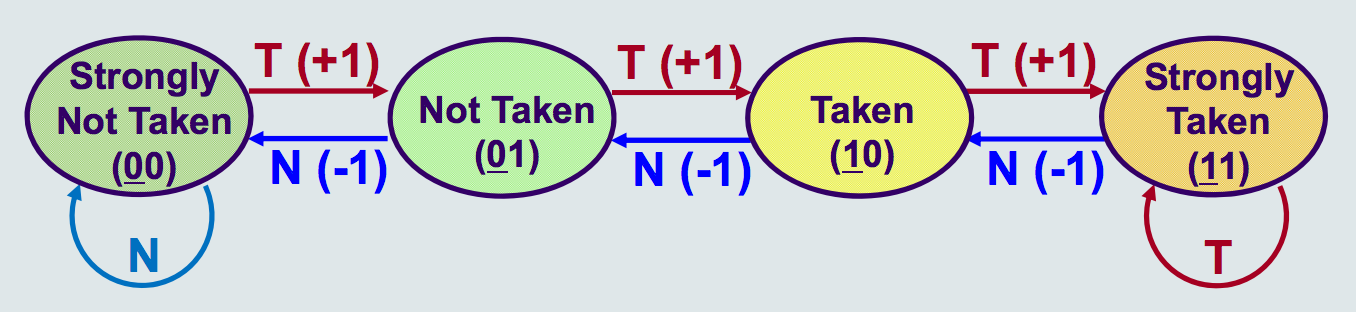
\includegraphics{img/bimodal-prediction.png}}
	\caption{Bimodal prediction using a 2-bit counter, much like a state diagram.}
	\label{fig:bimodal-prediction}
\end{figure}

\newpage
\section{Lecture 4: RISC Computers}
\subsection{Introduction}

\textbf{Reduced Instruction Set Computer (RISC)} represents an important innovation in computer architecture. It is an attempt to produce more computation power by simplifying the instruction set of the CPU.

The opposed trend to RISC it the \textbf{Complex Instruction Set Computer} (CISC), or ``the regular computers''.

Both these architectures have been developed to address problems caused by the \textbf{semantic gap}, which is the increasing gap between high level languages (e.g. Java, C++, C\#) and low level machine language.

\subsubsection{Main features of CISC}

\begin{itemize}
\item CISC attempts to make machine language (ML) instructions similar to high level languages (HLL)
\item Uses a large number of instructions aswell as complex instructions.
\item Many and complex addressing modes.
\item Microprogramming techniques are used to implement the complicated instructions.
\item Memory bottleneck is a major problem, due to complex addressing modes and multiple memory accesses instruction.
\end{itemize}

\subsubsection{Arguments for CISC}

\begin{itemize}
\item A rich instruction set should simplify the compiler by having instructions who match the HLL instructions.
\item Programs are smaller in size and will thus take up less of the memory and smaller execution time due to fewer instructions.
\item Program execution efficiency is improved by implementing complex operations in microcode rather than machine code.
\end{itemize}

\subsubsection{Microprogrammed Control}
Microprogramming is a technique used to implement the control unit.
\begin{itemize}
\item The basic idea is to implement the control unit as a microprogram execution machine (a computer inside a computer). \\
  -- The set of micro-operations occurring at one time defines a microinstruction. \\
  -- A sequence of microinstructions is called a microprogram. \\
\item The execution of a machine instruction becomes the execution of a sequence of micro-instructions. \\
  -- This is similar to that a C++ statement is implemented by a sequence of machine instructions.
\end{itemize}

\todo{Jag tror det är såhär en Olle Roos-dator fungerar med sitt mikrominne, FRÅGA YNGVE} \\
Microcodes are stored in a micromemory which is much faster than a cache, a ROM is often used because we almost never change this memory. Sometimes these memories are called firmwares.

\subsubsection{Problems with CISC}
As mentioned earlier, with CISC we simplify the compiler, but the hardware goes the opposite way and needs to be more complex. If complex instructions doesn't match the HLL instruction, in which case they may be of little use, this problem is getting bigger and bigger due to that the number of HLL are increasing.

A complex hardware design makes the release time of a processor longer.

\subsection{Program execution features}
what are programs doing most of the time? \\
Frequency of machine instructions executed:
\begin{itemize}
\item Moving data, 33\%
\item Conditional branches  20\%
\item Arithmetic/logic operations  16\%
\item Others  0.1-10\%
\end{itemize}

The majority of instructions uses simple addressing modes, complex addressing modes are only used by $\sim$18\%.

Operand types:
\begin{itemize}
\item 74-80\% scalars (integers, reals, characters, etc.).
\item the rest (20-26\%) are arrays/structures; 90\% of them are global variables
\item about 80\% of the scalars are local variables
\end{itemize}

\textbf{Conclusion}: The majority of operands are local variables of scalar type, which can be stored in registers.

For HLL statements, most of the time is spent executing CALLs and RETURNs in programs. Even though those only take up 15\% it still takes up most of the time due to long executing times for those two.

\subsection{RISC characteristics}
\begin{itemize}
\item Small number of simple instructions (desirable $\leq$ 100).
\item Execution of one instruction per clock cycle.
\item Complex operations are executed as a sequence of simple instructions.
\item only LOAD and STORE instructions reference data in memory.
\item Only a few simple addressing modes are used.
\item Instructions are of fixed length and uniform format.
\item Large number of registers, this is because the reduced complexity of the processor leaves silicon space on the chip to implement them (opposite of CISC).
\end{itemize}

\subsubsection{Register Windows}
Large number of registers is usually very useful. However, if contents of all registers must be saved at every procedure call, more registers mean longer delay. A solution to this problem is to divide the register file into a set of fixed-size windows. \\
-- Each window is assigned to a procedure. \\
-- Windows for adjacent procedures are overlapped to allow parameter passing \\

\subsubsection{Main advantages of RISC}
Best support is given by optimizing most used and most time consuming architecture aspects.
\begin{itemize}

\item Frequently executed instructions.
\item Simple memory reference.
\item Procedure call/return.
\item Pipeline design. \\
\end{itemize}

Consequently, we have:
\begin{itemize}
\item High performance for many applications:
\item Less design complexity.
\item Reduced power consumption.
\item reducing design cost and time-to-market (newer technology).
\end{itemize}
  
\subsubsection{Criticism of RISC}
\begin{itemize}
\item Operation might take several instructions to accomplish.
\item more memory access might be needed.
\item Execution speed may be reduced for certain applications.
\item It usually leads to longer programs, which needs larger memory space to store.
\item It makes it more difficult to program machine codes and assembly programs.
\end{itemize}
  
\subsection{RISC vs. CISC}
Studies have shown that RISC machines often run faster than CISC machines. But there is a problem in deciding what makes RISC better, some say it's not the hardware and instead the compilers for RISC that makes them better. But RISC on the other hand needs more memory because of its simpler instructions.

Most recent CPUs are not strictly RISC or CISC, but more hybrids of both.

In embedded systems RISC is \textbf{always} the better choice, due to:
\begin{itemize}
\item RISC gives better MIPS/watt ratio.
\item RISC reduces power consumption.
\item RISC lowers heat dissipation.
\item RISC simplifies hardware and its design.
\end{itemize}

ARM processors with RISC architecture have been widely used in smart phones and computers (e.g., iPad).


\newpage
\section{Lecture 5: Superscalar Architecture (SSA)}
Computer designed to improve computation on scalars instructions.
A scalar is a variable that can hold only one atomic value at a time, e.g., an integer or a real.
A scalar architecture processes one data item at a time -- the computers we discussed up till now.
Examples of non-scalar variables:
\begin{itemize}
\item Arrays -- Vector Processor
\item Matrices -- Graphics Processing Unit (GPU)
\item Records
\end{itemize}

In a superscalar architecture (SSA), several scalar instructions can be initiated simulaneously and executed independently.

\subsection{Instruction-level parallelism}
Most operations are on scalar quantities, speed up these operations will lead to large performance improvement.

\subsubsection{Superpipelining}
Superpipelining exploits the fact that many pipeline stages perform tasks that require less than half a clock cycle. Thus, a doubled internal clock speed allows the performance of two tasks in one external clock cycle.

We divide pipelining stages into several sub-stages, and hence increase the number of instructions which are handled by the pipeline at the same time. But note that although several instructions are executing concurrently, only one instruction is in its execution stage at any one time.

\todo{A picture would be nice here} \\

\begin{enumerate}
\item For example by diving each stage into two sub stages, we will be able (in the ideal situation) to perform each stage at twice the speed.
\item No duplication of hardware is needed. 
\item Not all stages can be divided into (equal length) sub stages.
\item Hazards more difficult to resolve.
\item More complex hardware.
\item Interrupt handling and testing will be more complicated.
\end{enumerate}
  
\subsubsection{Difference between Superpipelined and Superscalar Designs}
The difference is that Superpipeline can perform several instructions in one clock cycle, whereas Superscalar performs several instructions in parallel

\begin{figure}[H]
  \centering
  \scalebox{0.342}{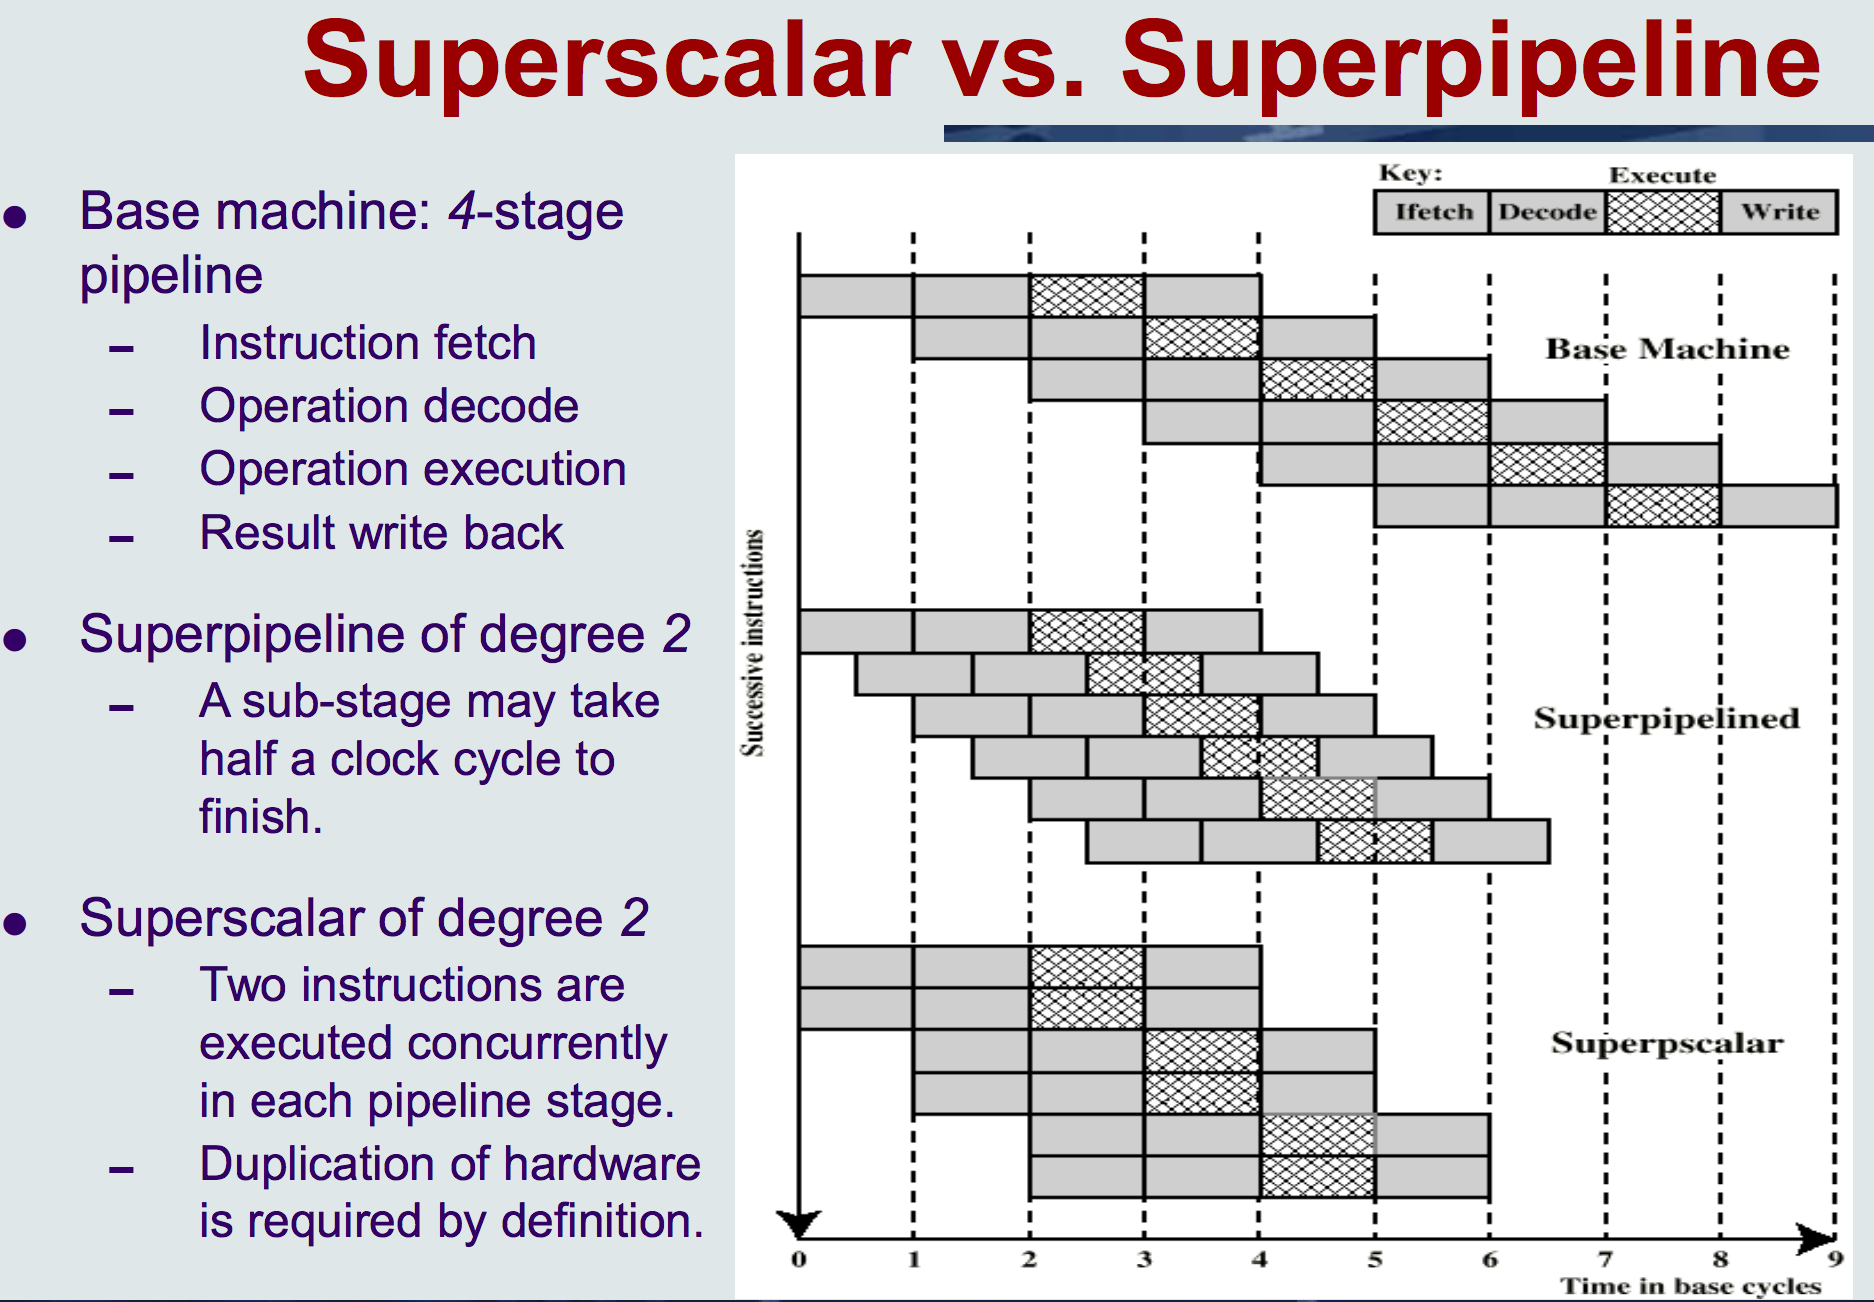
\includegraphics{img/superscalar-vs-superpipeline.png}}
  \caption{Difference between a Superscalar and a Superpipeline architecture}
  \label{fig:superscalar-vs-superpipeline}
\end{figure}


\subsubsection{Superscalar Superpipeline Design}

\begin{figure}[H]
  \centering
  \scalebox{0.342}{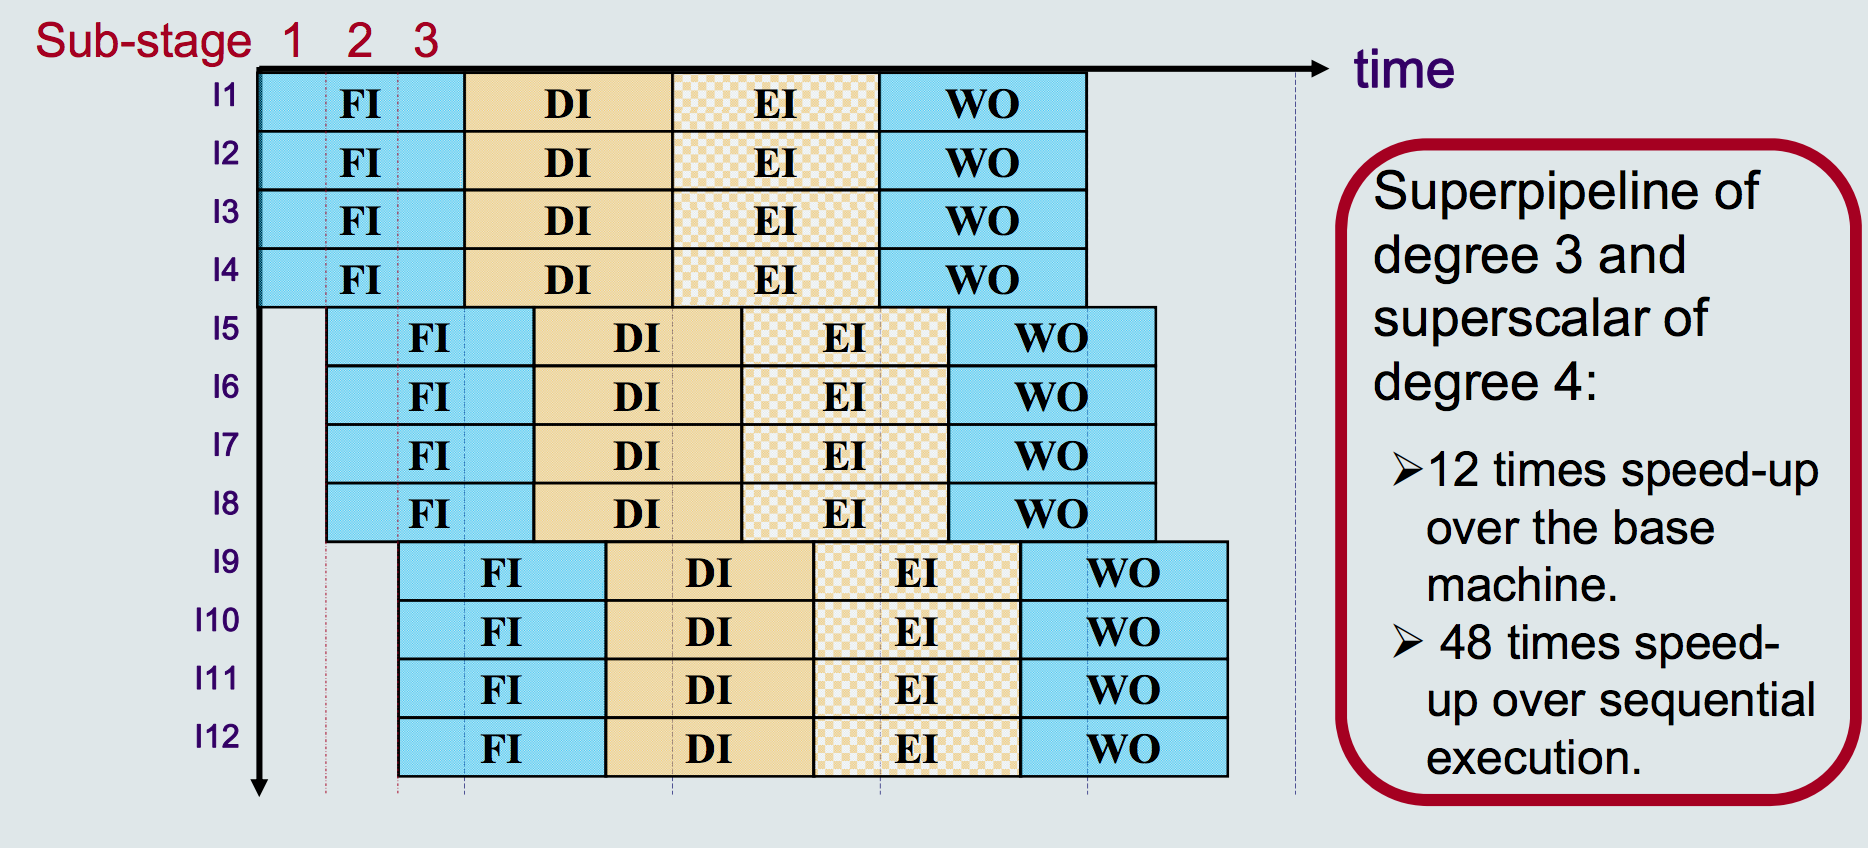
\includegraphics{img/superscalar-superpipeline.png}}
  \caption{Superscalar Superpipeline architecture}
  \label{fig:superscalar-superpipeline}
\end{figure}

The new trend is to combined the two ideas. In Figure \ref{fig:superscalar-superpipeline} it says that this would give us a 48 times speedup, this is not the case though because of data dependencies.

\subsection{Dependency issues}
The superscalar approach depends on the ability to execute multiple instructions in parallel. The term instruction-level parallelism refers to the degree to which, on average, the instructions of a program can be executed in parallel. A combination of compiler-based optimization and hardware techniques can be used to maximize instruction-level parallelism.

The main problems are:
\begin{itemize}
\item Resource conflicts.
\item Control (procedural) dependency.
\item Data dependencies.
\item True data dependency.
\item Output dependency.
\item Anti Dependency.
\end{itemize}
  
These are very similar to the cases in normal pipelining (data hazards). But the consequences are more severe here because the parallelism are greater and thus larger amount of performance will be lost.

\subsubsection{Resource Conflicts}
Several instructions compete for the same hardware resource at the same time.
\begin{itemize}
\item For instance, two aritmethic instructions need the same floating-point unit for execution.
\item similar to structural hazards in pipeline.
\end{itemize}

They can be solved \underline{partly} by introducing several hardware units for the same functions.
\begin{itemize}
\item e.g. have two floating point units.
\item the hardware units can also be pipelined to support several operations at the same time.
\item however, memory units \textbf{can't be duplicated}.
\end{itemize}
  
\subsubsection{Procedural Dependency}
The instructions following a branch (taken or not taken) have a procedural dependency on the branch and cannot be executed until the branch is executed.

As with regular pipelining, this type of procedural dependency also affects a scalar pipeline. The consequence for a superscalar pipeline is more severe, because a greater magnitude of opportunity is lost with each delay.

If variable-length instructions are used, then another sort of procedural dependency arises. Because the length of any particular instruction is not known, it must be at least partially decoded before the following instruction can be fetched. This prevents the simultaneous fetching required in a superscalar pipeline. This is one of the reasons that superscalar techniques are more readily applicable to a RISC or RISC-like architecture, with its fixed instruction length.

\subsubsection{Data Conflicts}
These are caused by dependencies between instructions in the program. They are similar to data hazards in regular pipelining, but they cause more problems due to that we much more data dependencies because of parallel execution of many instructions.

To address the problem and to increase the degree of parallel execution, SSA provides a great liberty in the order in which instructions are issued and executed. Therefore, data dependencies have to be considered and dealt with much more carefully.
\subsubsection{Window of execution}
Because of data dependencies, only some instructions are able to execute in parallel. The processor has to select from a sufficiently large instruction set. \textbf{Window of execution} is then the set of instructions that is considered to be able to execute in parallel at a certain moment.

The number of instructions in the window should be as large as possible, however it is limited by: \\
\begin{itemize}
\item Capacity to fetch instructions at a high rate.
\item The problem of branches.
\item The cost of hardware needed to analyze data dependencies (we don't really care about cost, we want to build cool stuff)
\end{itemize}

The window of execution can be extended over basic block borders by branch prediction (\textbf{speculative execution}).

\textbf{Speculative execution} works like this:
\begin{enumerate}
\item Instructions of the predicted path are entered into the window of execution.
\item If the prediction turns out to be correct, we were able to do some of them in advance (which is superduper), and the changes will become permanent and visible (they will \textbf{commit})
\item If not, all changes will undone, and the result will be ignored.
\end{enumerate}

\subsubsection{Data Dependencies}
All instructions in the window of execution may begin execution, subject to data dependence and resource constraints.
\begin{itemize}
\item True data dependency
\item Output dependency
\item Anti dependency
\end{itemize}

\subsubsection{True Data Dependency}
True data dependencies exist when the output of one instruction is required as an input to a subsequent instruction:
\begin{lstlisting}[frame=single]  % Start your code-block
  . . .
  MUL R4,R3,R1 (R4 := R3 * R1)
  . . .
  ADD R2,R4,R5 (R2 := R4 + R5)
\end{lstlisting}
In this example we can fetch and decode the second instruction in parallel, but we have to wait to perform it because its dependant on registers from the first instruction.

They are intrinsic features of a program, and cannot be eliminated by compiler or hardware techniques. The hardware have to detect them, and solve them. The easiest way to do this in this example, is just to stall the first instruction until we can perform the second.

This type of depency is very common, and by increasing the window size we can reduce the impact of them. \\

\subsubsection{Anti Dependency}
Also known as write after read, occurs when an instruction requires a value that is later updated. In the code block below, instruction 2 is anti-dependant on instruction 3. The ordering of the instructions cannot be changed, nor can the instructions be executed in parallel. 
\begin{lstlisting}[frame=single]  % Start your code-block
  . . .
  1. B = 3
  2. A = B + 1
  3. B = 7
\end{lstlisting}

Anti-dependcies are naming dependencies, renaming of variables could remove the dependency, as seen in the code below. \\

\begin{lstlisting}[frame=single]  % Start your code-block
  . . .
  1. B = 3
  N. B2 = B
  2. A = B2 + 1
  3. B = 7
\end{lstlisting}

\subsubsection{Output Dependency}
An output dependency, also known as write-after-write (WAW), occurs when the ordering of instructions will affect the final output value of a variable. In the example below, there is an output dependency between instructions 3 and 1 — changing the ordering of instructions in this example will change the final value of A, thus these instructions cannot be executed in parallel.

\begin{lstlisting}[frame=single]  % Start your code-block
  . . .
  1. B = 3
  2. A = B + 1
  3. B = 7
\end{lstlisting}

As with anti-dependencies, output dependencies are name dependencies. That is, they may be removed through renaming of variables, as in the below modification of the above example:

\begin{lstlisting}[frame=single]  % Start your code-block
  . . .
  1. B2 = 3
  2. A = B2 + 1
  3. B = 7
\end{lstlisting}

\subsection{Parallel instruction execution}
\textbf{Instruction-level parallelism (ILP)} is the average number of instructions in a program that a processor might be able to execute at the same time. It is determined by the number of \underline{true dependencies} and procedural (control) dependencies in relation to the number of other instructions.

Consider the following two code fragments. The three instructions on the left are independent, and in theory all three could be executed in parallel. In contrast, the three instructions on the right cannot be executed in parallel because the second instruction uses the result of the first, and the third instruction uses the result of the second.
\begin{lstlisting}[frame=single]  % Start your code-block
  . . .
  1. R1 = R2		1. R3 = R3 + 1
  2. R3 = R3 + 1	2. R4 = R4 + R2
  3. R4 = R4 + R2	3. R4 = R0
\end{lstlisting}

Instruction-level parallelism is also determined by operation latency: the time until the result of an instruction is available for use as an operand in a subsequent instruction. The latency determines how much of a delay a data or procedural dependency will cause.

\textbf{Machine parallelism} of a processor, is the ability of the processor to take advantage of the ILP of the program. It it determined by the number of instructions that can be fetched and executed at the same time (the number of parallel pipelines), and by the speed and sophistication of the mechanisms that the processor uses to find independent instructions.

The use of a fixed-length instruction set architecture, as in a RISC, enhances instruction-level parallelism. On the other hand, limited machine parallelism will limit performance no matter what the nature of the program.

To achieve high performance, we need both ILP and machine parallelism. Ideally, we have the same ILP and machine parallelism. However, this is impossible, since the same computer is used for programs with different ILPs. 

\subsubsection{Division and Decoupling}
To increase ILP, we should divide the instruction execution into smaller tasks and decouple them. In particular, we have three important activities:
\begin{itemize}
\item \textbf{Instruction Issue} -- an instruction is initiated and starts execution
\item \textbf{Instruction issue} -- an instruction is initiated and starts execution
\item \textbf{Instruction commit} -- the operation results are written back to the register files or cache (The machine state is changed).
\end{itemize}


\subsubsection{SSA instruction Execution Policies}
Instructions can be executed in an order different from the strictly sequential one, with the requirement that \textbf{the results must be the same}.

Execution policies usually used:
\begin{itemize}
\item In-order issue with in-order completion.
\item In-order issue with out-of-order completion.
\item Out-of-order issue with out-of-order completion.
\item \st{Out-of-order issue with in-order completion}.
\end{itemize}

\subsubsection{In-Order Issue with In-Order Completion}
Instructions are issued in exact program order, and completed in the same order (with parallel issue and completion, of course!).
\begin{itemize}
\item An instruction cannot be issued before the previous one has been issued.
\item An instruction cannot be completed before the previous one has been completed.
\end{itemize}

To guarantee in-order completion, an instruction will stall when there is a conflict and when a unit requires more than one cycle to execute.

\textbf{Example}: A processor can issue and decode 2 instructions per cycle, has 3 functional units (2 single-cycle integer units, and 1 two-cycle floating-point unit), and can write back 2 results per cycle.

An instruction sequence with the following characteristics:

\begin{itemize}
\item I1 – needs two execute cycles (floating-point)
\item I2 –
\item I3 –
\item I4 – needs the same function unit as I3
\item I5 – needs data value produced by I4
\item I6 – needs the same function unit as I5
\end{itemize}

\begin{figure}[H]
  \centering
  \scalebox{0.5}{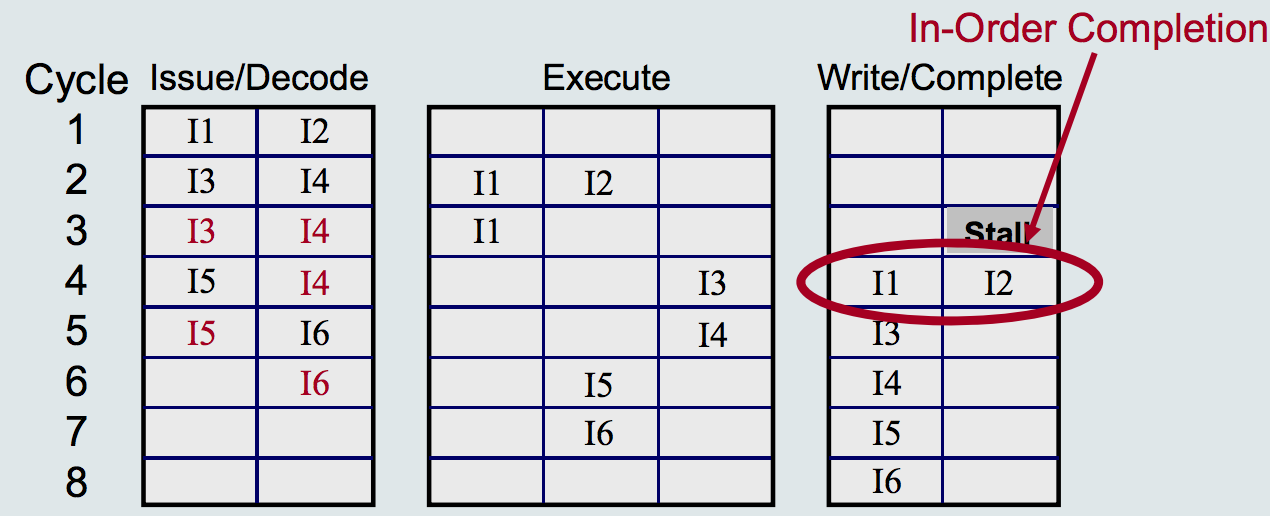
\includegraphics{img/IOI-IOC.png}}
  \caption{An example of In-Order Issue with In-Order Completion}
  \label{fig:IOI-IOC}
\end{figure}

The processor detects and handles (by stalling) true data dependencies and resource conflicts, and thus does not rely on compiler-based technique (compatibility consideration)

This is not a very efficient technique, but it simplifies the hardware.

\subsubsection{In-Order Issue with Out-of-Order Completion}
With out-of-order completion, a later instruction may complete before a previous one. It addresses mainly the issue of long-latency operations, such as division.

With out-of-order completion, any number of instructions may be in the exe- cution stage at any one time, up to the maximum degree of machine parallelism across all functional units. Instruction issuing is stalled by a resource conflict, a data dependency, or a procedural dependency.

\textbf{Example}:

\begin{itemize}
\item I1 – needs two execute cycles
\item I2 –
\item I3 –
\item I4 – conflict with I3
\item I5 – depending on I4
\item I6 – conflict with I5
\end{itemize}

\begin{figure}[H]
  \centering
  \scalebox{0.5}{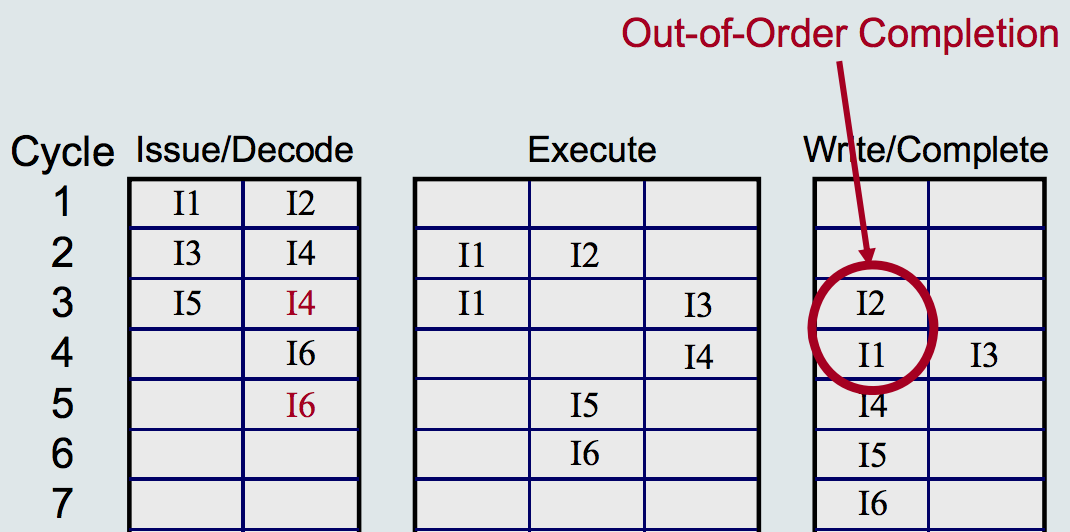
\includegraphics{img/IOI-OOC.png}}
  \caption{An example of In-Order Issue with Out-Order Completion}
  \label{fig:IOI-OOC}
\end{figure}

Now instruction I2 can write back, and doesn't have to wait for I1.
\todo{\\tror inte jag fattar det här rätt, kanske borde skriva om detta. \\ det står bättre i kursboken (runt sida 580), kanske borde skriva om det istället}

\subsubsection{Out-Order Issue with Out-of-Order Completion}
With \textbf{in-order issue}, no new instruction can be issued when the processor has detected a conflict, and is stalled until after the conflict has been resolved. The processor is not allowed to look ahead for further instructions, which could be executed in parallel with the current ones.

With \textbf{out-of-order issue} we can continue to fetch new instructions even though we have to stall in a later stage.

We can do this by decouple the decode and execution stages of the pipeline. We then use a buffer, called the \textbf{instruction window} which we put the instructions in when we have fetched and decoded them, note that this can only be done if this buffer if not full.

When an functional unit becomes free, an instruction from the instruction window may be issued to the execution stage. Any instruction may be issued as long as it is of the right type for the free unit, and it doesn't inflict any conflict.

\textbf{Example}:

\begin{itemize}
\item I1 – needs two execute cycles
\item I2 –
\item I3 –
\item I4 – conflict with I3
\item I5 – depending on I4
\item I6 – conflict with I5
\end{itemize}

\begin{figure}[H]
  \centering
  \scalebox{0.5}{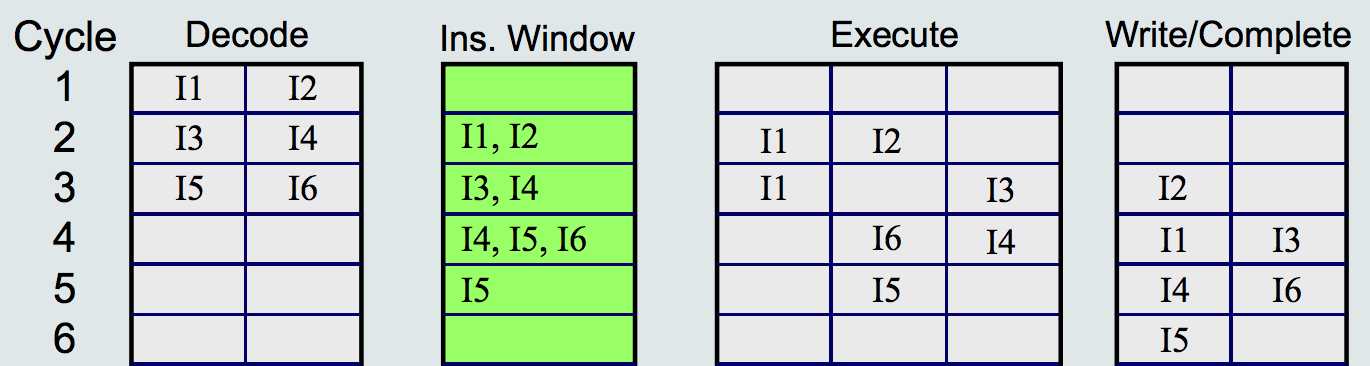
\includegraphics{img/OOI-OOC.png}}
  \caption{An example of Out-Order Issue with Out-Order Completion}
  \label{fig:OOI-OOC}
\end{figure}

This works as a look-ahead capability for the processor. Instructions are issued from the instruction window with little regard for their original program order. As before, the only constraint is that the program execution behaves correctly.

\todo{\\det står mer om detta i kursboken också sida 583-584}

\newpage
\section{Lecture 6: VLIW Processors}
The difference from Superscalar is that in that architecture the hardware solves everything for us, if improvements are made on the design we don't need to change the programs. \\
The down side though is that the architecture is very complex. \\
-- A lot of hardware is needed for run-time detection of parallelism. \\
-- It consumes a lot of power. \\
-- There is, therefore a limit in how far we can go with this technique. \\

The instruction window for execution is limited in size. \\
-- This limits the capacity to detect large number of parallel instructions.

\subsection{Very Long Instruction Word Processors}
Several operations that can be executed in parallel are placed in a single instruction word. \\
--VLIW rely on compile-time detecton of parallelism. \\
-- The compiler analyzes the program and detects operations to be executed in parallel. \\

After one instruction has been fetched, all the corresponding operations are issued in paralell.
The instruction window limitation disappears: the compiler can potentially analyze the whole program to detect parallel operations.

\subsubsection{Explicit Parallelism}
Instruction parallelism scheduled at compile time.\\
-- Included within the machine instructions explicitly.\\

An EPIC (Explicitly Parallel Instruction Computing) processor \\
--uses this information to perform parallel execution. \\

The hardware is very much simplified \\
-- The controller is similar to a simple scalar computer. \\
-- The number of FUs can be increased without needing additional sophisticated hardware to detect parallelism, as in SSA. \\

Compiler has much more time to determine parallel operations. \\
-- This analysis is only done once off-line, while run-time detection is carried out by SSA hardware for each execution of the code. \\
--Good compilers can detect parallelism based on global analysis of the whole program. \\

\subsubsection{Main issues}
-- Need a large number of registers. \\
-- Large data transport capacity is needed between Fus and the register files and between register files and memory. \\
-- High bandwidth between instruction cache and fetch unit is also needed due to long iunstructions.

\subsubsection{Software issues}

\subsection{Loop unrolling}

\subsection{IA-64 architecture}
\subsubsection{Predicated execution}
\subsubsection{Instruction format}
\subsubsection{Branch Predication}
\textbf{NOT THE SAME AS BRANCH PREDICTION}
\subsubsection{Placement of Loading}
\subsubsection{Speculative Loading}


\newpage
\section{Lecture 7: Parallel Processing}
\subsubsection{Why Parallel Processing?}
\subsubsection{Parallel Computer}
\subsubsection{Parallel Program}
\todo{Allt det här känns som repetition, borde jag skippa?}

\subsection{Architecture classification}
\subsubsection{Flynn’s Classification of Architectures}
\begin{itemize}
\item Single instruction, single data stream - \textbf{SISD} \\
\item Single instruction, multiple data stream - \textbf{SIMD} \\
\item Multiple instruction, single data stream - \textbf{MISD} \\
\item Multiple instruction, multiple data stream- \textbf{MIMD} \\
\end{itemize}

\subsubsection{SISD}
The regular computers who use a single processor, a single instruction stream, and stores data in a single memory.
\subsubsection{SIMD}
Computers with multiple processing elements that perform the same operation on multiple data points simultaneously. There are simultaneous (parallel) computations, but only a single process (instruction) at a given moment.

Array and vector processors are the most common examples of SIMD machines.
\subsubsection{MISD}
Computers where many functional units perform different operations on the same data.
\begin{figure}[H]
  \centering
  \scalebox{0.6}{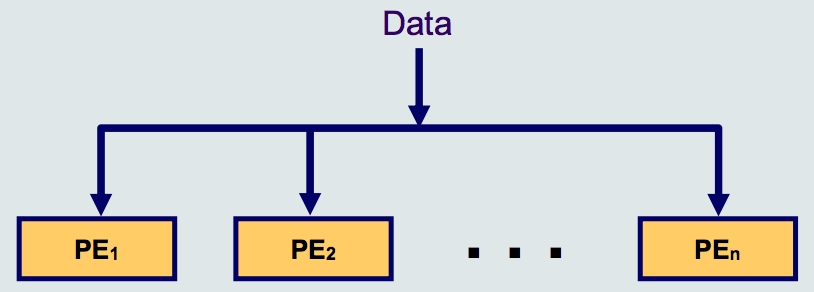
\includegraphics{img/MISD.png}}
  \caption{MISD architecture}
  \label{fig:MISD}
\end{figure}

\subsubsection{MIMD}
A set of processors that simultaneously perform different instructions sequences, on different sets of data.

There is also different classes of MIMD computers:
\begin{itemize}
  \item Shared memory (tightly coupled).
  \begin{itemize}
  \item Symmetric multiprocessor (SMP).
  \item Non-uniform memory access (NUMA).
  \end{itemize}
  \item Distributed memory (loosely coupled) = Clusters.
\end{itemize}

\begin{figure}[H]
  \centering
  \scalebox{0.6}{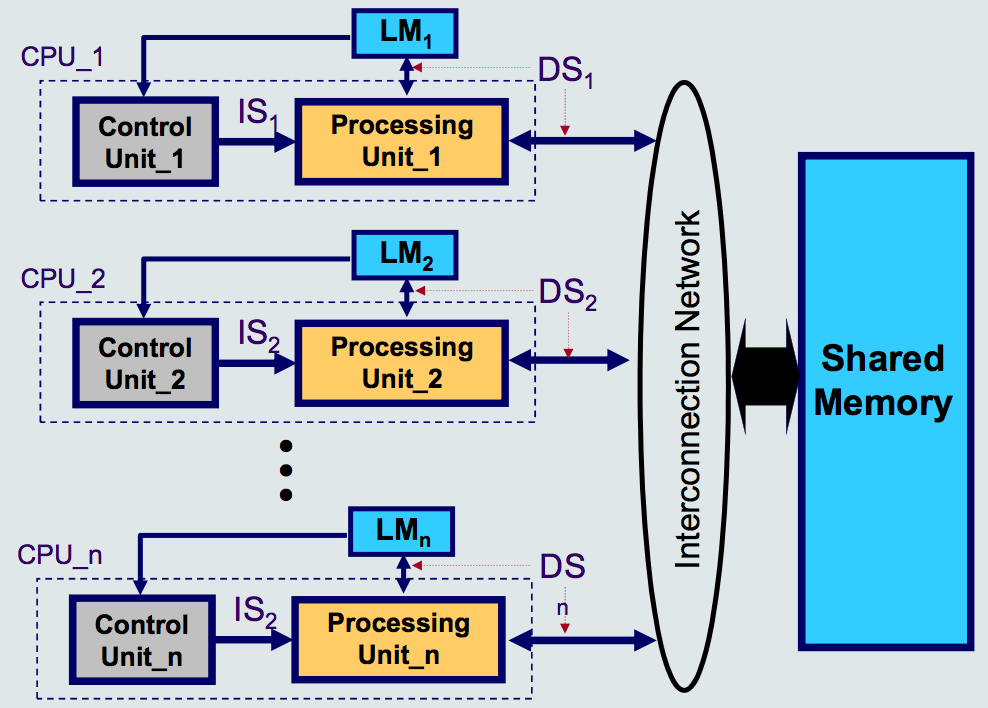
\includegraphics{img/MIMD.png}}
  \caption{MIMD architecture}
  \label{fig:MIMD}
\end{figure}

\subsection{Performance evaluation}
The peak rate of a computer is the maximum value that the computer can work at, this is something that vendors use to sell computers and not something that is really useful for us.

\textbf{Speedup}: measures the gain we get by using a parallel computer, over a sequential one, to run a given application

$$S = \frac{T_s}{T_p}$$

$T_s$ : execution time needed with the sequential computer. \\
$T_p$ : execution time needed with the parallel computer. \\

\textbf{Efficiency}: to relate speedup to the number of processors used, it provides therefore a measure of the efficiency with which the processors are used.

$$E = \frac{S}{P}$$

$S$: speedup. \\
$P$: number of processors. \\
For the ideal situation, in theory: $S = P$; which means $E = 1$.

\textbf{Practically the ideal efficiency of 1 cannot be achieved!}

\subsubsection{Amdahls Law}
Gives the theoretical speedup in latency of the execution of a task at fixed workload that can be expected of a system whose resources are improved.

$$S_{latency}(s)=\frac{1}{1-p+\frac{p}{s}}$$

where
\begin{itemize}
\item $S_{latency}$ is the theoretical speedup in latency of the execution of the whole task;
\item $s$ is the speedup in latency of the execution of the part of the task that benefits from the improvement of the resources of the system;
\item $p$ is the percentage of the execution time of the whole task concerning the part that benefits from the improvement of the resources of the system before the improvement.
  \newline
\end{itemize}

Furthermore:
\begin{equation*}
  \begin{cases}
    S_{latency}(s) \leq \frac{1}{1-p} \\
    \lim_{s \to \infty} = \frac{1}{1-p}
  \end{cases}
\end{equation*}

show that the theoretical speedup of the execution of the whole task increases with the improvement of the resources of the system and that regardless the magnitude of the improvement, the theoretical speedup is always limited by the part of the task that cannot benefit from the improvement.

Amdahl's law is often used in parallel computing to predict the theoretical speedup when using multiple processors. For example, if a program needs 20 hours using a single processor core, and a particular part of the program which takes one hour to execute cannot be parallelized, while the remaining 19 hours (p = 0.95) of execution time can be parallelized, then regardless of how many processors are devoted to a parallelized execution of this program, the minimum execution time cannot be less than that critical one hour. Hence, the theoretical speedup is limited to at most 20 times (1/(1 -- p) = 20). For this reason parallel computing is relevant only for a low number of processors and very parallelizable programs. This can be seen in figure \ref{fig:amdahls-law}

\begin{figure}[H]
  \centering
  \scalebox{0.6}{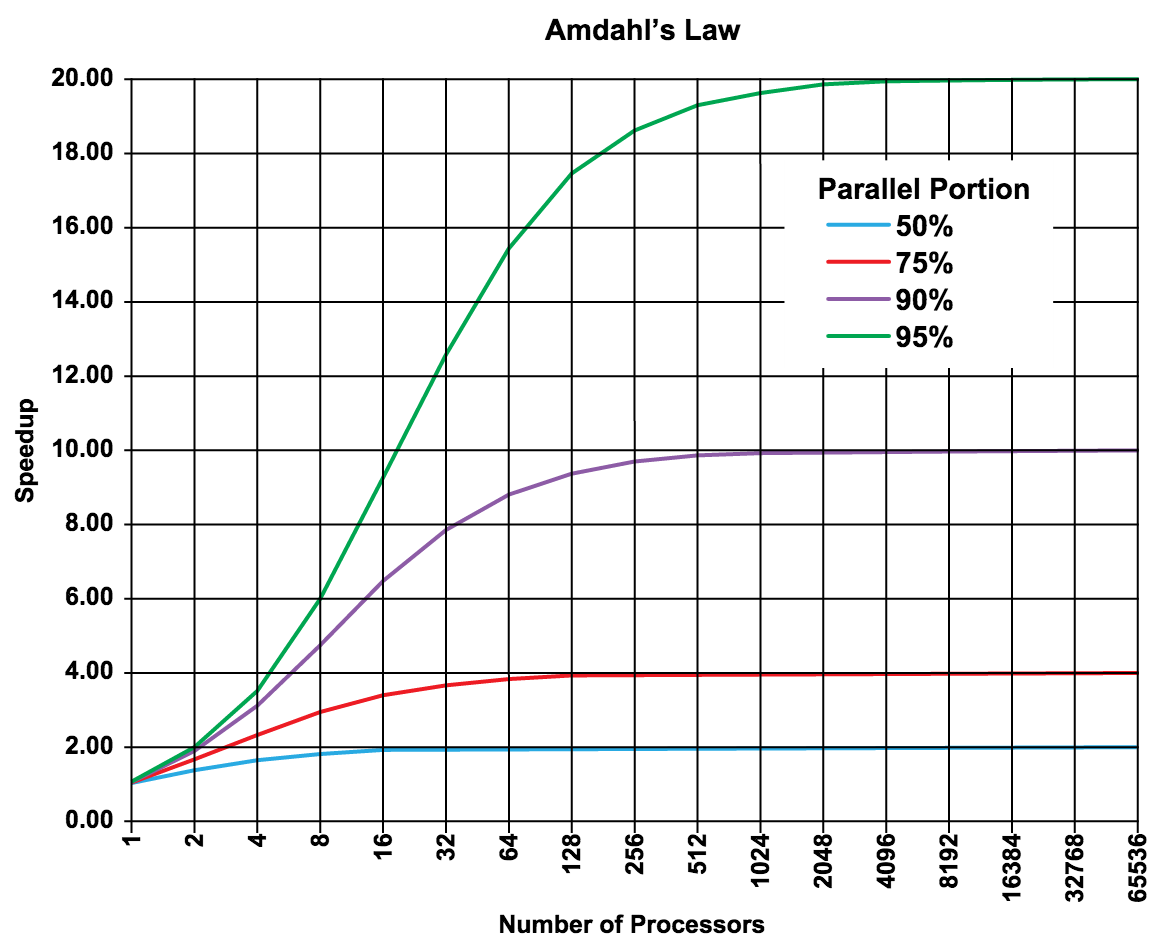
\includegraphics{img/amdahls-law.png}}
  \caption{Amdahls Law}
  \label{fig:amdahls-law}
\end{figure}

\todo{skipped other factors that limit speedup} \\
\todo{and impact of communications}

\subsection{Interconnection network}
\subsubsection{Single Bus}
\subsubsection{Completely Connected Network}
\subsubsection{Crossbar Network}
\subsubsection{Mesh Network}
\subsubsection{Hypercube Network}

\newpage
\section{Lecture 8: SIMD Architectures}

\subsection{Vector Processors}
-- array processors \\
-- vector processors \\
-- data parallelism \\
Typical SISD processors who behave like SIMD processors

\subsubsection{Instruction-level parallelism}
\subsubsection{Thread-level parallelism}
\subsubsection{Data parallelism}
\subsubsection{Vector Processors}
\subsection{Array Processors}
Typical SIMD processors

\subsection{Dedicated Memory Organization}
\subsection{Global Memory Organization}
\subsection{Cray supercomputers}
\subsubsection{Cray X1}
\subsection{Multimedia extensions}
\subsubsection{sub-word execution}
\subsubsection{Packed Data Types}
\subsubsection{SIMD Arithmetic Examples}

\newpage
\section{Lecture 9: MIMD Architectures}
A set of general purpose processors connected together \\
In contrast to a SIMD computer, a MIMD computer can execute different programs on different processors. \\

-- Works asynchronously, and don't have to synchronize with each other. \\
-- At any time, different processors may be executing different instructions on different pieces of data. \\
-- They can be built from commodity (off-the-shelf) microprocessors with relatively little effort. \\
-- They are also highly scalable, provided that an appropiate memory organization is used. \\
-- Most current parallel computer are built based on the MIMD architecture. \\

\subsubsection{SIMD vs. MIMD}
\subsubsection{MIMD Processor Classification}
\subsubsection{MIMD with Shared Memory}
\subsubsection{MIMD with Distributed Memory}
\subsubsection{Shared-Address-Space Platforms}
\subsubsection{Multi-Computer Systems}
\subsubsection{MIM Design Issues}
\subsection{Symmetric multiprocessors (SMP)}
\subsubsection{SMP Advantages}
\subsubsection{SMP based on Shared Bus}
\subsubsection{Multi-Port Memory SMP}
\subsubsection{Operation System Issues}
\subsubsection{IBM S/390}
\subsection{NUMA Architecture}
\subsubsection{Memory Access Approaches}
\subsection{Clusters}
\subsubsection{Losely Coupled MIMD - Clusters}
\subsubsection{Clusters benefits}
\subsubsection{Clusters Configurations}
\subsubsection{IBM Blue Gene Supercomputer}
\subsubsection{Parallelizing Computation}
\subsubsection{Google Applications}

\newpage
\section{Lecture 10: Cache Coherence}
To many section without text seems to bug \LaTeX
\subsection{Introduction}
\subsubsection{Write Through}
\subsubsection{Write Back}
\subsubsection{Software Solutions}
\subsubsection{Hardware Solutions}
\subsection{Directory protocols}
\subsubsection{Cache Coherence Operations}
\subsection{Snoopy protocols}
\subsubsection{Write Invalidate SP}
\subsubsection{Snoopy Cache Organization}
\subsubsection{MESI State Transition Diagram}
\subsubsection{Write Update SP}
\subsubsection{Invalidate vs. Update Protocols}
\subsubsection{Directory vs. Snoopy Schemes}
\subsection{L1-L2 consistence}
\subsubsection{Alpha-Server 4100}

\newpage
\section{Lecture 11: Multi-Core and GPU}
To many section without text seems to bug \LaTeX
\subsection{Multi-Core Computers}
\subsubsection{Intel Core i7}
\subsubsection{Superscalar vs. Multi-Core}
\subsubsection{Single Core vs. Multi-Core}
\subsubsection{Intel Polaris}
\subsection{Multithreading}
\subsubsection{Thread-Level Parallelism (TLP)}
\subsubsection{Scalar Processor Approaches}
\subsubsection{Superscalar Approaches}
\subsubsection{SMT and Chip Multiprocessing}
\subsubsection{Multithreading Paradigms}
\subsection{Graphic Processing Unit (GPU)}
\subsubsection{CPU vs. GPU}
\subsection{General Purpose GPUs}
\subsubsection{Divergent Execution}
\subsubsection{Reduce Branch Divergence}
\subsubsection{GPUPU}
\subsubsection{NVIDIA Tesla}
\subsubsection{CUDA Programming Language}

\newpage
xb\section{Lecture 12: Low Power Architecture}
For some applications, low power consumption is more important than performance:
\begin{itemize}
\item Mobile communication and computing
\item Wirteless internet
\item Medical implants
\item Deep space applications 
\end{itemize}

Low-power designs will lead to:
\begin{itemize}
\item Longer battery life time
\item Lower cost (Cooling and package, Electricity bill)
\item Higher reliability and longer life time (due to lower temperature and smaller temperature gradients).
  \newline
\end{itemize}

\begin{figure}[H]
  \centering
  \scalebox{0.5}{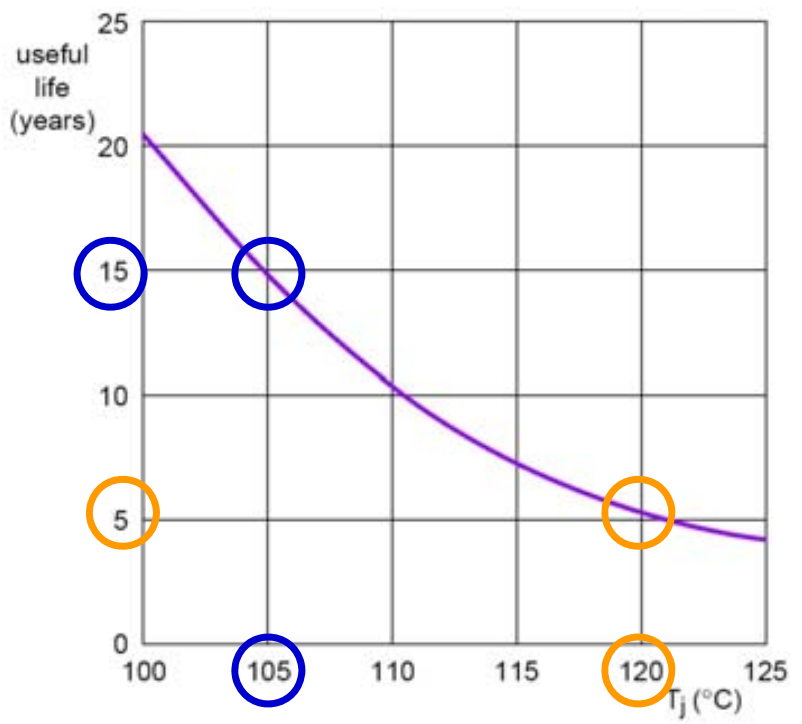
\includegraphics{img/thermal-reliability.png}}
  \caption{How the temperature affects the lifespan of a processor.}
  \label{fig:thermal-reliability}
\end{figure}

\subsection{Low-Power Techniques}
What can we do to reduce power consumption. At a low level we can use sign-magnitude representation over two complements representation for integer, this is because when using twos complement and switching between positive and negative numbers, almost all bits needs to be switched as can be seen in figure \ref{fig:2comp-vs-sign}

\begin{figure}[H]
  \centering
  \scalebox{0.5}{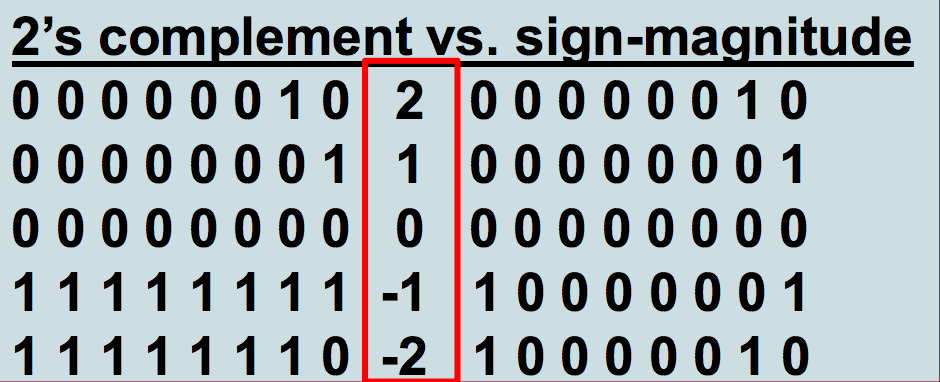
\includegraphics{img/2comp-vs-sign.png}}
  \caption{two's complement vs sign-magnitude representation.}
  \label{fig:2comp-vs-sign}
\end{figure}

We can also optimize with software such as:
\begin{itemize}
\item Use power efficient algorithms.
\item Compiler to optimize for more power efficient code.
\item Run-time power management by the OS.
\end{itemize}


\subsection{Design for low power \todo{kanske kan plocka bort denna och låta allt stå under första rubriken}}
\subsection{The Cursoe Processors}
\subsection{The ARM Processors}
\subsection{Final remarks}


\end{document}

